\chapter{Experiencias realizadas (mediciones)}
\section{Implementación en software}
\subsection{Reed-Solomon}
\subsection{Bloom-filter}
\subsection{Simulador de ruido óptico}
%% de orte.text
The physical optical channel simulation block provides an estimate of
the BER performance of the optical channel. Simulation steps are as
follows: RZ upstream traffic coming from all ONUs is assumed to arrive
at the $128\times1$ splitter with perfect time synchronization, i.e., there is no timing jitter. 
%This allows to simulate merged traffic as a simple addition of optical intensities at bit slots for either `0' or `1' bits. % borrar!
The `0'-bit slots contain a small CW optical intensity given by the Tx extinction ratio. 
Each on-line ONU adds its `0'-bit optical intensity yielding a base power level.
% As many bit `0' optical intensities are added as on-line ONUs to produce a base power level.  
Each `1'-bit adds a super-Gaussian ($m=4$) pulse, duty cycle $1/3$, to the base power level. %, with rising edge at slot start and peak amplitude accordingly to Tx optical mean output power.
% As many bit `1' intensities are added to base level as active Tx there are at each simulation bit slot.
 
Upstream and downstream merged traffic suffers from attenuation due to
splitter, fiber, and
splice losses. The power budget is balanced by an EDFA with $27$~dB constant gain.
Amplified spontaneous emission from the EDFA is modeled by white Gaussian
noise, with intensity proportional to the amplifier noise figure ($7$~dB), and is added
after the EDFA. 

%Real EDFAs gain increases with higher input power, i.e. amplification is not
%linear with number of active Txs. Settling for worst case scenario simulation
%we assume same $27\,dB$ gain for any number of active Txs. ASE noise produced
%at EDFA is modelled as a white Gaussian noise added to the optical signal. An
%EDFA accomplishing the amplification previously discussed ($-25.5\,dBm$ to
%$1.5\,dBm$) would have an output SNR $\geq 60\,dB$ accordingly to a estimation
%based on the bandwidth of forthcoming optical filtering at APD detector (see
%section 6.5.1 at~\cite{Agrawal:xx}). Dispersion compensation regeneration stage
%operation is accounted for by simulating no dispersion effects. Traffic is
%routed back to all ONUs by a 1x128 splitter through another $10\,km$
%fiber,
%amounting to a $27.5\,dB$ attenuation; so for one active Tx input power at each
%Rx would be $-27\,dBm$.

The input optical signal at the receiver is filtered (2nd order low-pass Butterworth filter, $25$~GHz bandwidth) and photodetected assuming a standard PD responsivity (see section 4.4.3 of~\cite{Agrawal:xx}).
White Gaussian noise accounting for thermal and shot noise is then added
to the photocurrent, and 
electrical filtering is applied (2nd order low-pass Butterworth filter, $14$~GHz bandwidth).
%Simulating the decision process a mean of samples around maximum eye opening is compared to a threshold current. 
%Current in case of `1' bits collision is higher than that of a single active Tx, so threshold is established assuming that later case.

%Real EDFAs gain increases with higher input power, i.e., amplification would not be linear with number of active Txs. 
%Settling for worst case scenario simulation we assume same $27\,dB$ gain for any number of active Txs. 
%ASE noise produced at EDFA is modeled as a white Gaussian noise that's added to the electric field. 
%An EDFA accomplishing the amplification previously discussed ($-25.5\,dBm$ to  $1.5\,dBm$) would have an output SNR $\geq 100\,dB$ accordingly to a estimation based on the bandwidth of forthcoming optical filtering at detector (see section 6.5.1 at~\cite{Agrawal:xx}). 
%Effect on traffic of dispersion compensation regeneration stage is accounted by not including in the simulation pulses deformation due to dispersion. 
%Afterwards traffic is routed back to all ONUs by a $1\times128$
%splitter through another $10\,km$ fiber, amounting to a $27.5\,dB$ attenuation arriving to each Rx with $-27\,dB$ for one active Tx.
%
%A concern was if maximum mean total input power allowed at Rx would be surpassed when multiple Tx were simultaneously active. 
%Simulation shown that the occurrence of 15 simultaneously active Tx was a very rare event {\bf <CUANTO??>}. 
%That would amount to $\sim-15\,dBm$ reaching each ONU Rx, well bellow standard commercial Rx overload of $\sim+0.5\,dBm$, that's maximum acceptable mean input power for a BER$<1\,10^{-12}$. 
%
%Rx optical bandwidth is simulated as a low pass filter (2nd order Butterworth as a digital IIR filter~\cite{IIR}, cutoff frequency $25\,GHz$). Afterwards optical traffic is converted into an electrical current. Then to account for thermal and shot noise at a typical APD white Gaussian noise current is added, with an estimated SNR $\simeq 42\,dB$ (see section 4.4.3 at~\cite{Agrawal:xx}). Then electrical filtering is applied (2nd order Butterworth IIR filter, cutoff frequency $6\,GHz$). Detection procedure is performed by comparison to a fixed current threshold. A previous simulation run with the same number of ONUs but with a single active Tx allows to determine the decision threshold at the time of maximum eye diagram opening. Addition of bit `1' amplitudes (collision) produce a current even higher than for a single active Tx, thus this bit slot will be classified as `1' at optical channel simulation output. 
%Media block account for fiber, EDFA and splitters. It attenuates optical trains (splitters and fiber attenuation minus EDFA gain) and also adds white Gaussian noise to the electric field accounting for ASE noise at EDFA. 
% MUCHO, MUY IMPORTANTE: REVISAR CALCULO OSNR (Fn) y verificar que se determina en detector %[VAB]
% ITU recommendation G. 959.1 states that certain interfaces' should operate normally up to $12\,dBm$ mean total input power. In any case if such power is surpassed it would only cause a very short time blinding of Rx affecting a so small amount of bits that wouldn't affect the logical layer ability to correct them.
% receiver overload: max input power for BER<1E-12
%Receiver block simulates Rx behavior. It's optical bandwidth is taken into account by simulating a low pass filtering of incoming traffic (2nd order Butterworth as a digital IIR filter~\cite{IIR}, cutoff frequency $25\,GHz$). Then optical traffic is converted into an electrical current. White Gaussian noise current is added to account for thermal noise at Rx, being it's SNR $\simeq 42\,dB$ accounting for thermal and shot noise at a typical APD detector (see section 4.4.3 at~\cite{Agrawal:xx}). Afterwards another filter simulates detector's linear channel (2nd order Butterworth IIR filter, cutoff frequency $6\,GHz$). Detection procedure is performed by comparison to a fixed current threshold. A previous simulation run with same number of ONUs but with a single active Tx allows to determine the decision threshold at the time of maximum eye diagram opening. Addition of bit `1' amplitudes (collision) produce a current even higher than for a single active Tx, thus this bit slot will be classified as `1' at 
optical channel simulation output. 


%\section{Simulation results}
Noise fluctuations at power levels near the PD sensitivity limit have an important effect on signal detection. 
%Detection being made at power levels near PD sensitivity is highly sensitive to changes in noise.
Shot noise is of particular concern as it is proportional to the mean photocurrent.
In our network proposal the later is higher than in PONs as bit
`0' optical intensities from all ONUs are added.
The resulting base-level optical intensity is then heavily dependent on the Tx extinction ratio.
Fig.~\ref{sim:optical} shows minimal extinction ratios required to
achieve an arbitrary BER in the physical layer as a function of the
number of on-line ONUs.
\begin{figure}[!t]
    \centering
      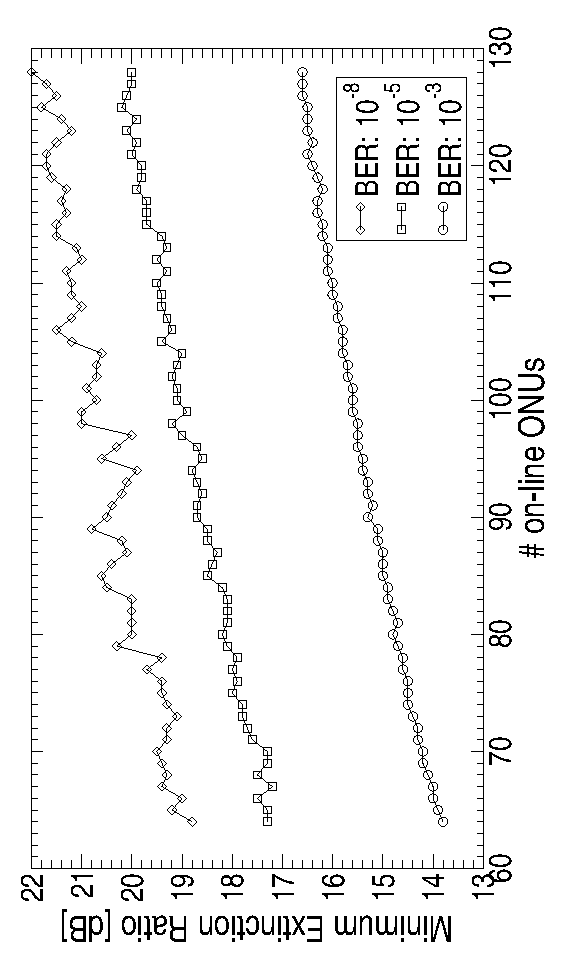
\includegraphics[angle= 270, width=3.5 in]{orte03.pdf}
      \caption{Physical layer simulation result: Minimal extinction ratio required to assure a given BER}
      \label{sim:optical}
\end{figure}
In the $128$ ONUs scenario a  BER$<10^{-3}$ can be achieved using
commercially available transmitters with an extinction ratio $\simeq16.6$~dB.
This BER is low enough to allow for logical-channel error-correction routines that guarantee error-free transmission, while still making use of a fair fraction of channel capacity.
% perform correctly and still use a fair fraction of channel capacity.
% Fig.~\ref{sim:optical} shows simulation results for the BER vs OSNR
% for different numbers of ONUs with fixed electrical SNR $\simeq 42$~dB.
% Higher BERs as ONUs number increases due to the higher probability of
% simultaneous bit `1' transmissions (collisions) yielding pulses of
% optical power higher than that of a logical
% `1', generating intersymbol interference. Higher powers generate higher
% currents at Rxs that demand longer times to settle to logical `0' levels after
% filtering. Nevertheless, as
% can be seen in fig.~\ref{sim:optical}, in the worst case scenario (128
% ONUs) the expected OSNR at the EDFA output is enough ($\geq 40$~dB) to
% ensure a BER$<10^{-7}$. In this case simulation shown that the occurrence of
% 15 simultaneously active Tx was a very rare event, so optical power at Rx
% would be $\simeq -15$~dBm, well bellow standard commercial Rx overload
% of $\sim0.5$~dBm (maximum acceptable mean input power for a
% BER$<10^{-12}$).
\begin{figure}[!t]
    \centering
      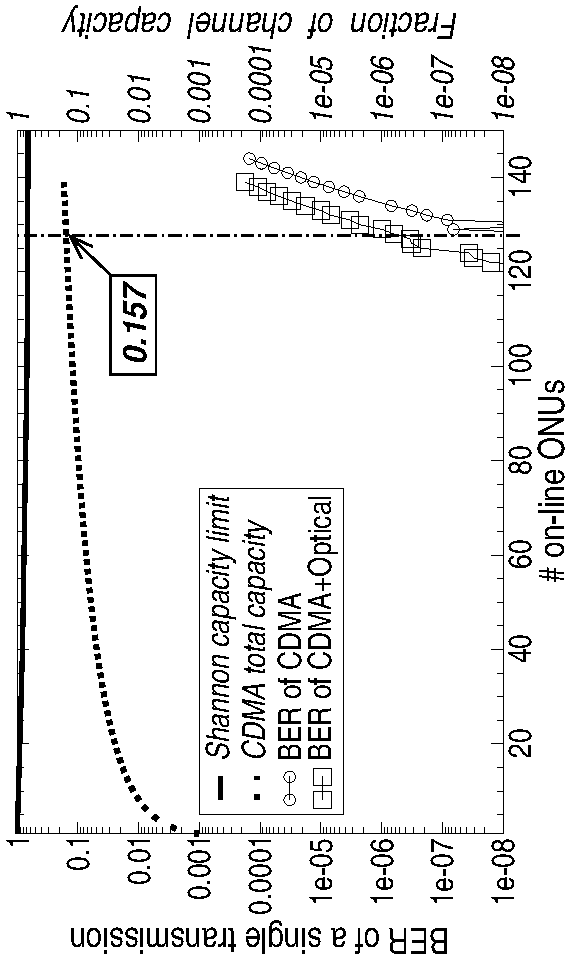
\includegraphics[angle=270 ,width=3.5 in]{orte04.pdf}
    \caption{Simulation results: Logical channel}
      \label{sim:access}
\end{figure}
Fig.~\ref{sim:access} shows simulation results for the fraction of the total
capacity and the BER of one channel at the coding level (circles) and 
including physical layer impairments (squares). These results were obtained by
sending one Gigabit of data for each ONU simultaneously.
This figure shows a channel utilization of $15.7\%$ when all of $128$ ONUs
are transmitting simultaneously, with a BER$<10^{-8}$. 
From Fig. \ref{arch:fig1} we observe a penalty of $8$ ONUs when
impairments from the optical layer (mainly extinction ratio and noise from EDFA and PDs) are taken into account.
Considering that the system was designed to support asynchronous communications (e.g., Ethernet), it is not likely that all the ONUs will transmit simultaneously (e.g., Internet links often operate at most at $90\%$ load); and therefore our system has a BER $<10^{-8}$ for each channel when 119 ONUs are transmitting at a same time ($119/128>0.9$).
%, removing only one ONU re-establish the desired BER. 
%
%It is worth to remark that, even if the optical channel can induce a
%significant number of errors, the access layer has shown to be able to correct a
%very large number of errors (it is based on
%LDPC+Reed-Solomon+Bloom-Filters), as can be seen on the curve with squares
%at fig.~\ref{sim:access}.
Observe that the high error rates correspond to a
worst-case scenario when all ONUs are transmitting simultaneously at
full capacity, and also 
there is a low penalty due to physical layer impairments.
%Figure~\ref{sim:optical} presents the simulation's BER vs optical OSNR
%for different numbers of ONUs. %[VAB]
%As the number of ONUs increases higher BERs are obtained at the same optical SNR (electrical SNR is fixed at $\simeq 42\,dB$). In particular there is a penalty of about $30\;dB$ for 128 ONUs in comparison to 1 ONU. This is expected as a consequence of the higher probability of simultaneous bit `1' transmissions (collisions) yielding pulses (logical `1's) of different powers (sum of the power of each transmitter). Higher powers demand more time to settle post filtering current to logical `0' levels. If the following bit slot is indeed a logical `0' an erroneous determination is more possible with a higher collision probability. Nevertheless it can be inferred from simulation results that optical channel should not add significantly to the BER for the whole link as the estimated optical SNR of $\geq 100\,dB$ even for the worst case scenario with 128 ONUs present.
% \begin{figure}[!t]
%     \center
% %     \subfigure[Optical channel]{
% %      \label{sim:optical}
%       \includegraphics[scale=0.4]{BERvsSNR_6GHz.pdf}
% %    }
% %    \subfigure[Logical channel]{
% %      \label{sim:access}
%       \includegraphics[scale=0.4]{BERvsONUs.pdf}
% %    }
%     \caption{Simulation results}
%       \label{archfig}
% \end{figure}

\section{Implementación en FPGA}
El estudio de PONs plantea el desafío de generar, transmitir y recibir
señales de 10 Gbps en el laboratorio. El costo de estos sistemas
suele ser muy elevado. En este trabajo proponemos una alternativa de muy
bajo costo basada en la generación y trasmisión de señales en FPGAs.

\subsection{Arquitectura alto-nivel de la FPGA Xilinx ML507}
El equipamiento consta de un kit de desarrollo ML-507 de Xilinx y un
transceptor SFP+ con láser de 1330 nm, con capacidad de hasta 10 Gbps
en modulación NRZ y alcance de 10km en fibra monomodo. Para realizar
las mediciones presentadas en este trabajo se utilizaron dos dispositivos:
\begin{itemize}
 \item {\em Integrated Bit Error Rate Tester} (iBERT) \cite{4gtxs}: Es
un medidor de tasa de error que utiliza un analizador lógico embebido dentro
del mismo diseño de la FPGA, con interfaz para la herramienta de
verificación y depuración ChipScope. Mediante este agregado, que debe
ser sintetizado dentro del diseño, es posible medir en tiempo real
varios parámetros del transceptor asi como realizar estadísticas y
mediciones de error, variando tasas y características de la transmisión
en tiempo real.
 \item Osciloscopio Óptico Agilent 86100A con módulo óptico 86105A: Para
realizar las mediciones físicas contamos con este equipo que posee un
ancho de banda de 20 Ghz en potencia óptica, suficiente para capturar en
tiempo real los bits individuales o realizar un diagrama de ojo.
\end{itemize}
\subsection{Transmisión a multi-gigabit}
\subsection{Diseño del sistema propuesto}
\section{Redes ópticas}
% de confEUA.tex

\subsection{Transmisión a 9 Gbps con SFP+}
El montaje para la experiencia se realizó conectando el transceptor SFP+
al conector correspondiente en la placa de desarrollo ML-507 y un bucle de
fibra óptica ({\em loopback}), con el objetivo de realizar las
mediciones de BER. Luego, para realizar las mediciones con el
osciloscopio, se debe conectar el extremo de recepción de la fibra
óptica al osciloscopio. En este caso generamos el disparo del
osciloscopio mediante la señal de reloj del sistema (placa ML-507) que
se obtiene a través de los conectores SMA J12 y J13 (si bien es
diferencial sólo utilizamos uno de ellos).  Para la depuración y
configuración se utilizó la interfaz JTAG USB de Xilinx ``Platform Cable
USB II''.
\subsection{Configuración del reloj del transceptor}

La tasa de transmisión del transceptor GTX está dada por la
frecuencia de reloj de entrada $F_{PLL\_Clock}$, donde se transmite un
bit por cada semiciclo (la modulación es NRZ); entonces la tasa de
transmisión será
$R_{line}\mbox{[bps]}=F_{PLL\_Clock}\mbox{[1/s]} \times 2$.  La
frecuencia del reloj de entrada del PLL está gobernada por la ecuación
5-1 \cite[Pag. 88]{ug198}, que reproducimos a continuación:

\begin{equation}
F_{PLL\_Clock} = F_{CLKIN} \times \frac{PLL\_DIVSEL\_FB \times
DIV}{PLL\_DIVSEL\_REF}% \enspace
\end{equation}\\

donde las constantes $PLL\_DIVSEL\_REF = \{1;2\}$, $DIV = \{4;5\} $ y
$PLL\_DIVSEL\_FB = \{1;2;3;4;5\}$ son configurables por software;
mientras que la frecuencia base se configura con las llaves
SW6~\cite[Tabla 1-32]{ug347}: $
F_{CLKIN} (Mhz)= \{62.5;75;77.76;100;125;150;156.25;311.04;622.08\}$.


 Modificando los parámetros puede lograrse, en teoría, un amplio rango
de la frecuencias $F_{PLL\_Clock}$, pero de acuerdo a la documentación
del PLL \cite[Pág. 71]{ug366}~\footnote{La velocidad máxima no se
detalla en la documentación del GTX de Virtex5, pero si en la
documentación del Virtex6, que excepto en el modelo HTX posee parámetros
similares.}, este tiene un rango de operación nominal desde $1.2$ a
$2.7$ Ghz en FPGAs de grado $-1$ tal como el que se encuentra en la
placa de desarrollo ML-507. Sin embargo en este artículo documentamos la
obtención y medición de velocidades de oscilación estables para el PLL
de hasta $4.5$ Ghz (lo que implica una tasa de transmisión de $9$ Gbps),
fuera del rango de operación especificado por el fabricante.

\begin{figure}[t]
  \centering
    %\includegraphics[scale=0.70]{plot.png}
    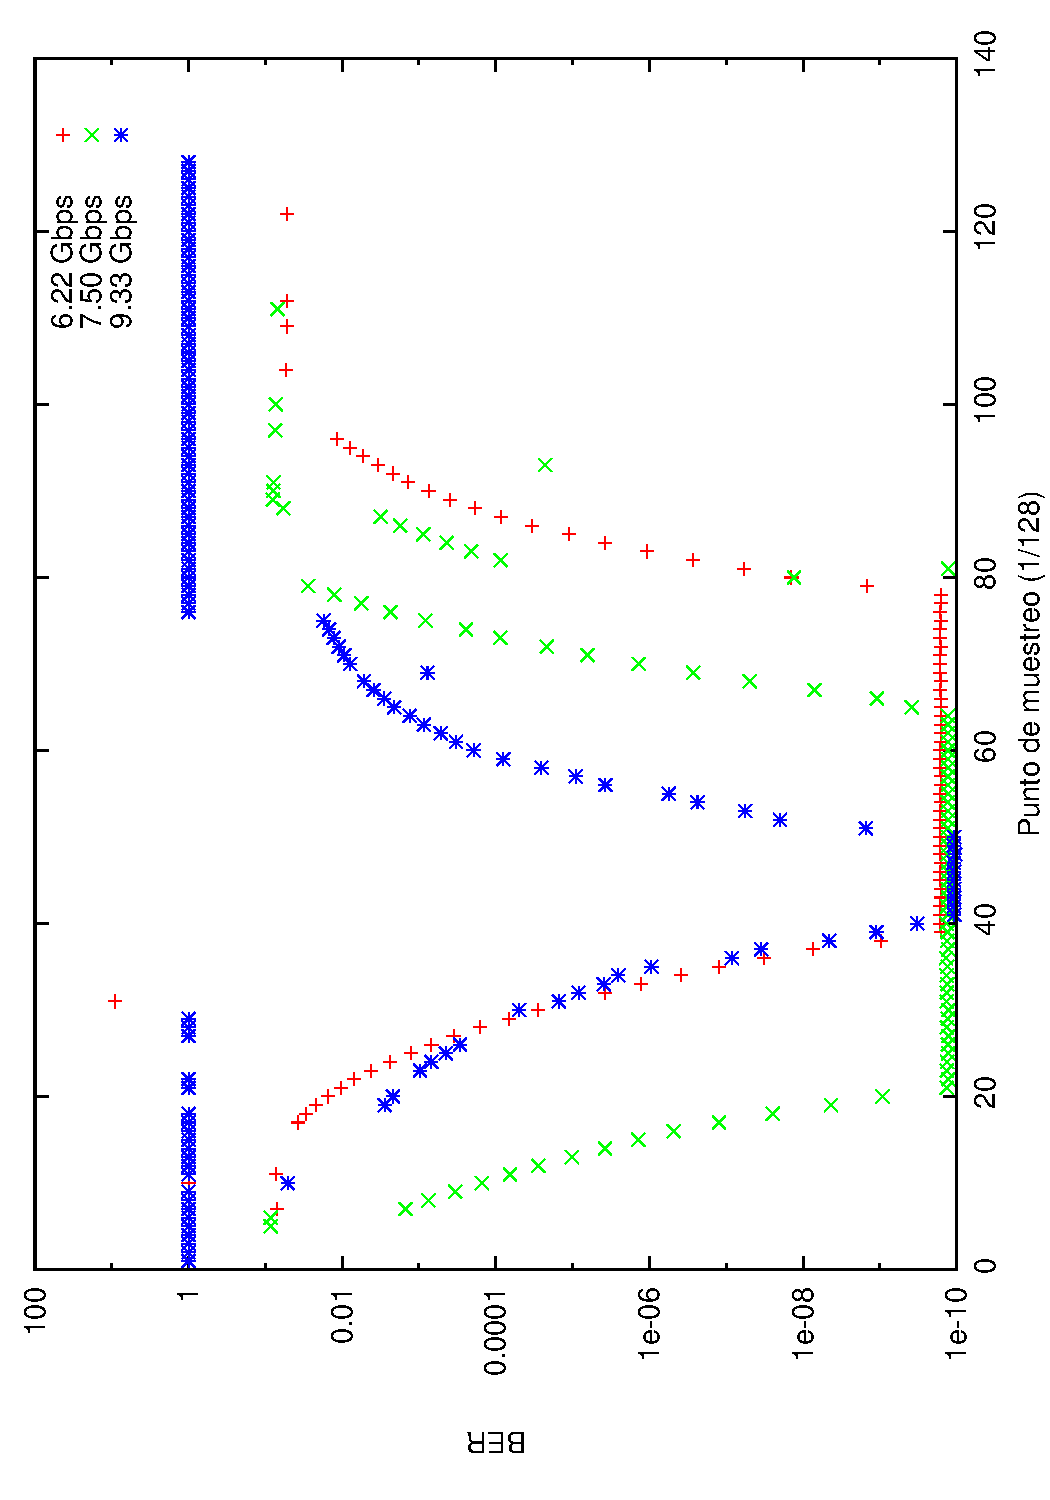
\includegraphics[width=6cm,angle=270]{medicionesPaper/BER_sp.pdf}
\caption {BER vs. punto de muestreo.}
\label{fig:BER}
\end{figure}

\section{Mediciones}
\begin{figure}[!t]
  \centering
%  \subfigure[$4.5$ Gbps]{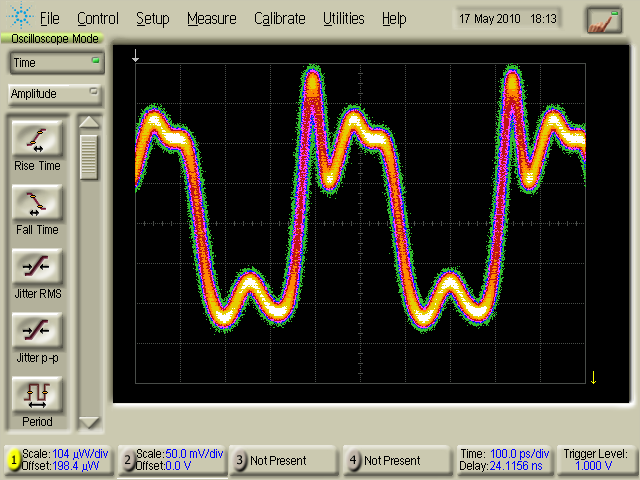
\includegraphics[scale=0.52]{medicionesPaper/screen3.png}
  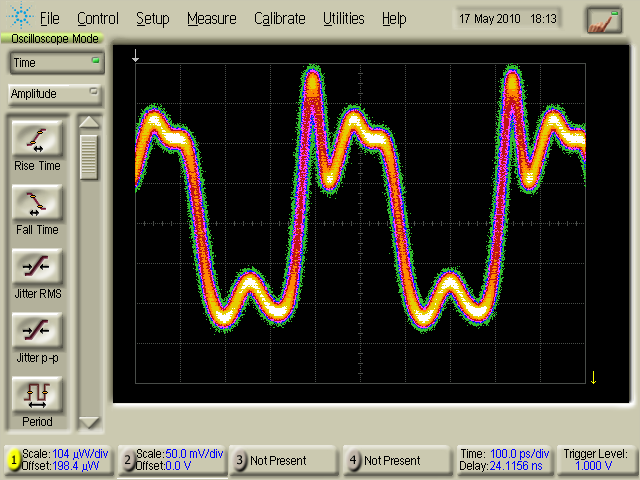
\includegraphics[scale=0.52]{medicionesPaper/screen3.png}
  \caption {Señal óptica a $4.5$ Gbps}
  \label{fig:Img1}
%  \\[1cm]
\end{figure}

\begin{figure}[!t]
  \centering
%  \subfigure[$6$ Gbps]{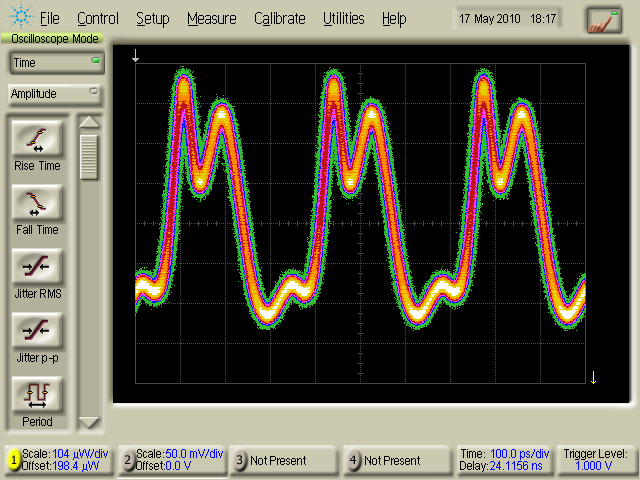
\includegraphics[scale=0.52]{medicionesPaper/screen4.png}
 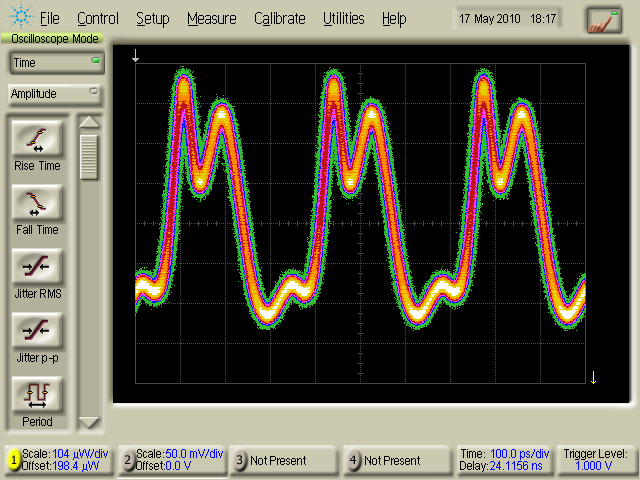
\includegraphics[scale=0.52]{medicionesPaper/screen4.png}
  \caption {Señal óptica a $6$ Gbps}
  \label{fig:Img2}
%  \\[1cm]
\end{figure}

\begin{figure}[!t]
  \centering
%  \subfigure[$7.5$ Gbps]{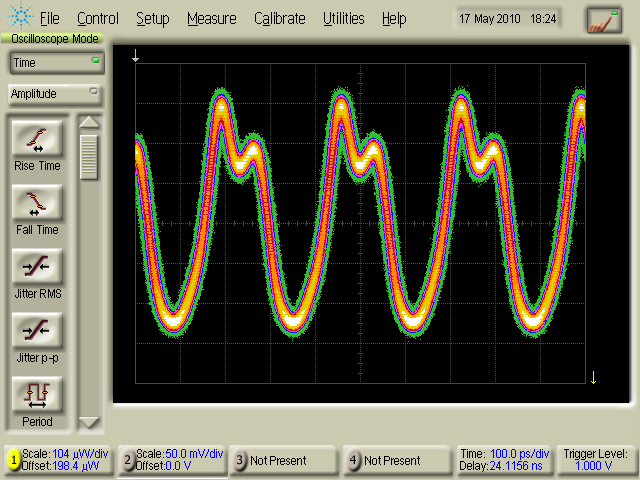
\includegraphics[scale=0.52]{medicionesPaper/screen5.png}
 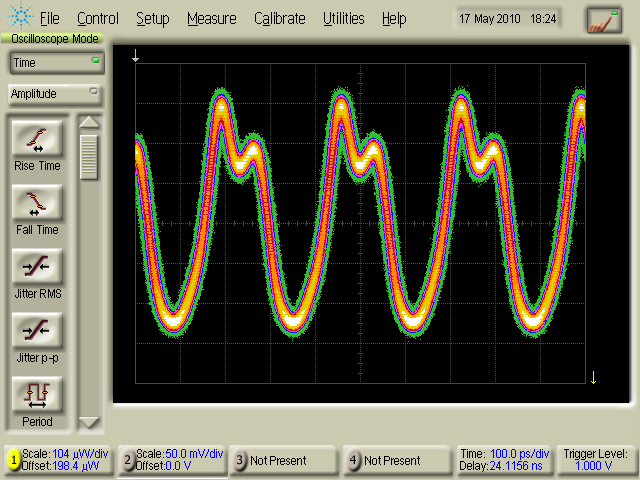
\includegraphics[scale=0.52]{medicionesPaper/screen5.png}
  \caption {Señal óptica a $7.5$ Gbps}
  \label{fig:Img3}
%  }
\end{figure}


\begin{figure}[!t]
  \centering
%  \subfigure[$9.33$ Gbps]{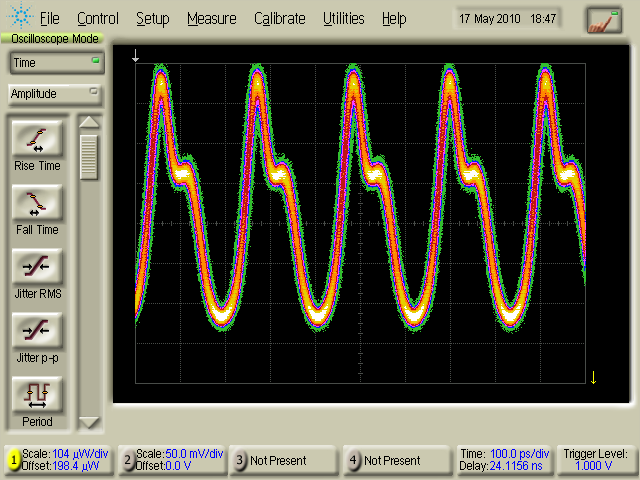
\includegraphics[scale=0.52]{medicionesPaper/screen6.png}
 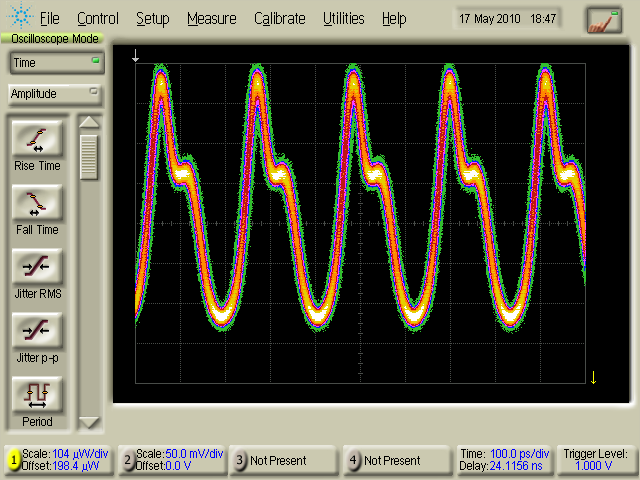
\includegraphics[scale=0.52]{medicionesPaper/screen6.png}
  \caption {Señal óptica a $9.33$ Gbps}
  \label{fig:Img4}
%  }\\[1cm]
\end{figure}


\begin{figure}[!t]
  \centering
%  \subfigure[$12.44$ Gbps]{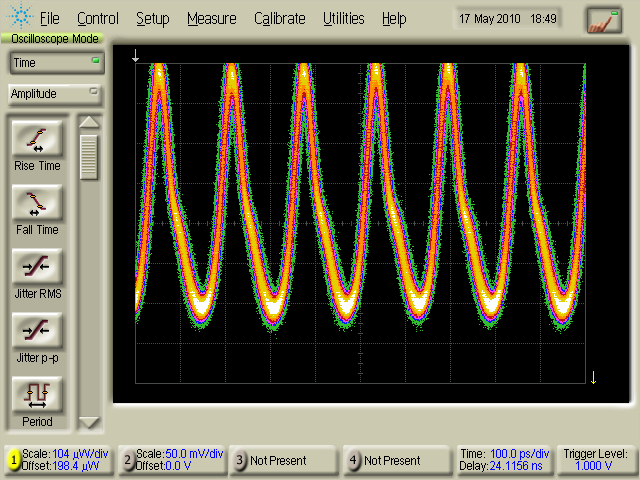
\includegraphics[scale=0.52]{medicionesPaper/screen7.png}
 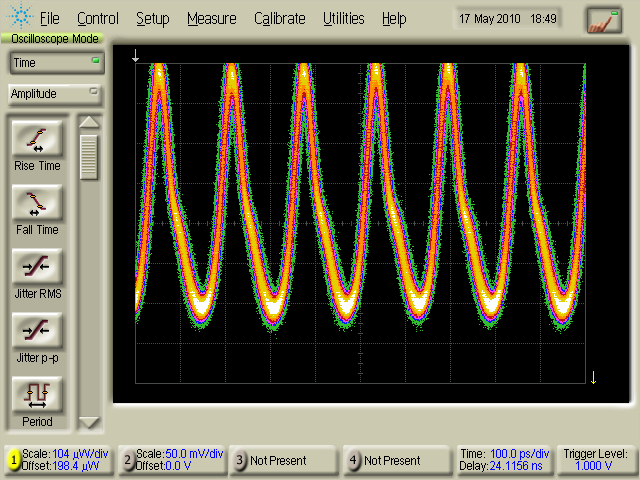
\includegraphics[scale=0.52]{medicionesPaper/screen7.png}
  \caption {Señal óptica a $12.44$ Gbps}
  \label{fig:Img5}
%  }
\end{figure}



\begin{figure}[!t]
  \centering
  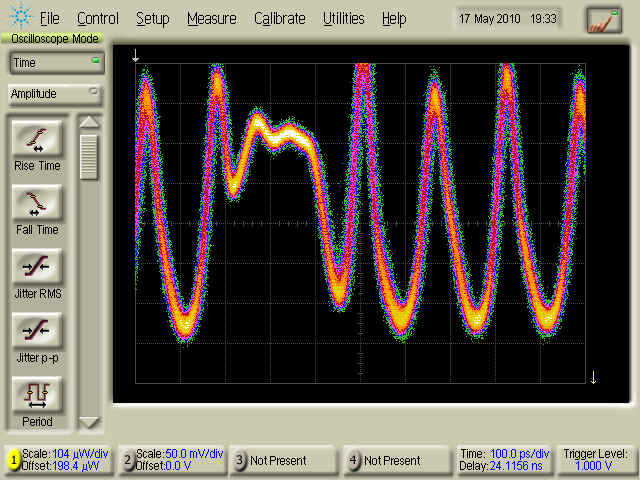
\includegraphics[scale=0.52]{medicionesPaper/screen12.png}
  \caption {Señal óptica a $12.44$ Gbps, transmisión 10110101010}
  \label{fig:Img6}
\end{figure}



Las figuras \ref{fig:Img1} a \ref{fig:Img5} muestran la señal óptica producida a diferentes
tasas. Nótese que aunque el equipo puede generar señales estables de
hasta $12.44$ Gbps pero no puede recibirlas a esa frecuencia, por lo que las
mediciones de BER se realizaron solo hasta $9.33$ Gbps. Todas las señales
corresponden a la secuencia 10101010, excepto la figura \ref{fig:Img6},
que fue generada con una secuencia distinta para demostrar el total
control sobre la señal generada. El transceptor posee la capacidad de
realizar una codificación 8B/10B adicional, pero para estas mediciones
ese módulo fue desactivado.



\subsection{Implementación del sistema sobre 8B/10B}
\section{Redes acústicas}
\subsection{Sincronización}
% de newJIS_140512
On-Off Keying modulation of sound waves, following the Z-channel interface model described in Section 2.2., encode the transmitted bits as pulses. Carrier frequency can vary from 10 kHz to 16 kHz. Good results can be obtained with a rate of 1000 bps at frame level. In experiments, delay (the time for a bit to traverse the network) was very high, due to Reed-Solomon 223/255 coding, a frame to support up to 16 users and the low capacity of the physical media. A more sensible choice of FEC algorithm (like BCH [12]) could drastically reduce data delay. Simple pulse shaping is realized using a pass-band filter at the output of the modulation and also at the input of the demodulator. This filter also helps reject unwanted interference.
As it follows from the description of the communication channel, synchronization between the transmitter and receiver is essential for the correct decoding of information. For this purpose, an initial synchronization pattern is sent, so the receiver can adjust parameters like phase and decision level (see Figure 3). For the data bits transmission a duty cycle of 50\% showed in our experiments an enhanced detection. Clock drift and jitter are not significant at this low transmission speed and so no correction is required, making the software modem implementation very simple. Decision level is dynamic, meaning it is constantly re-calculated from averaged input data. The receiver symbol phase is also corrected using the input data as reference. Notice that this simple synchronization method allows detecting the frame start as well as the bit slot; both are needed at every communication. Moreover, once the data began to be transmitted, the communication becomes indecipherable thanks to the CS-PRNG.

\subsection{Modulación}
\subsection{Medición multi-usuario}
\subsection{Medición distintas distancias}

\section{Conclusiones}